\section{New Pipeline}
\begin{frame}{New Pipeline}
\begin{figure}
        \centering
        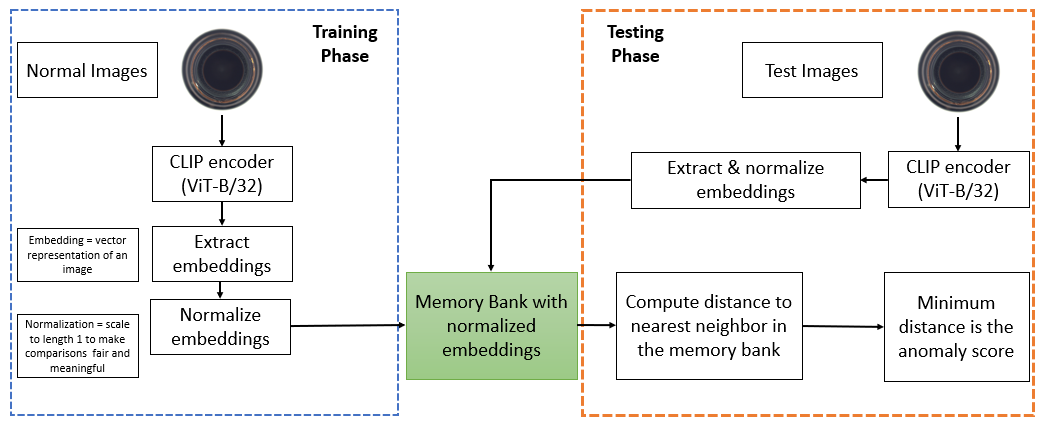
\includegraphics[width=\linewidth]{images/new_pipeline.png}
        \caption{New Pipeline with CLIP encoder}
    \end{figure}
\end{frame}
\begin{frame}{Information about CLIP encoder (ViT-B/32)}
  \begin{itemize}
    \item Vision Transformer (ViT) backbone used in CLIP.
    \item \textbf{B} = Base size (12 layers, hidden size 768, 12 heads).
    \item \textbf{/32} = Patch size $32 \times 32$.
    \item Processes images into patch tokens for transformer encoding.
  \end{itemize}
\end{frame}
% Input processing
\begin{frame}{Input Processing}
  \begin{itemize}
    \item Input image size: $224 \times 224$ pixels.
    \item Divided into $32 \times 32$ patches.
    \item Number of patches: $7 \times 7 = 49$.
    \item Plus one [CLS] token for global representation.
  \end{itemize}
\end{frame}

% Transformer architecture
\begin{frame}{Transformer Architecture}
  \begin{itemize}
    \item Each patch embedded into a 768-dim vector.
    \item 12 Transformer layers process the sequence.
    \item Self-attention captures global dependencies between patches.
    \item Final [CLS] token used as image representation.
  \end{itemize}
\end{frame}

% Output
\begin{frame}{Output Representation}
  \begin{itemize}
    \item Transformer output: 768-dim features.
    \item Projected to a 512-dim embedding space in CLIP.
    \item Embedding normalized (unit vector).
    \item Used for similarity with text embeddings or anomaly detection.
  \end{itemize}
\end{frame}
\begin{frame}{Dataset for Model and Dataset}
    Dataset for:
    \begin{itemize}
        \item Original PatchCore encoder dataset : ImageNet-1k.

        \item New VLM-PatchCore encoder(Vit B/32) dataset : LAION-2B.

        \item Both model evaluated on MVTec-AD.
    \end{itemize}
\end{frame}
\begin{frame}{Evaluation Metrics for Anomaly Detection}
\begin{itemize}
    \item \textbf{Image-level AUROC} 
    \begin{itemize}
        \item Measures ability to distinguish normal vs. anomalous images.
        \item ROC-AUC based on one score per image.
    \end{itemize}

    \item \textbf{Pixel-level AUROC} 
    \begin{itemize}
        \item Measures how well pixel-wise anomaly maps match ground-truth masks.
        \item Flatten heatmap vs. mask $\rightarrow$ ROC-AUC.
    \end{itemize}

    \item \textbf{PRO Score (Per-Region Overlap)} 
    \begin{itemize}
        \item Evaluates overlap between predicted anomaly regions and ground-truth.
        \item Robust to threshold choice.
    \end{itemize}

    \item \textbf{F1 / Dice (optional)} 
    \begin{itemize}
        \item Computed at best threshold.
        \item Balances precision (few false alarms) and recall (detect all anomalies).
    \end{itemize}

    \item \textbf{Runtime \& Memory Comparison}
    \begin{itemize}
        \item Training/inference time.
        \item Memory bank size (full vs. coreset).
    \end{itemize}
\end{itemize}
\end{frame}
\begin{frame}{Comparison between CNN and VLM backbone}
\begin{figure}
    \centering
    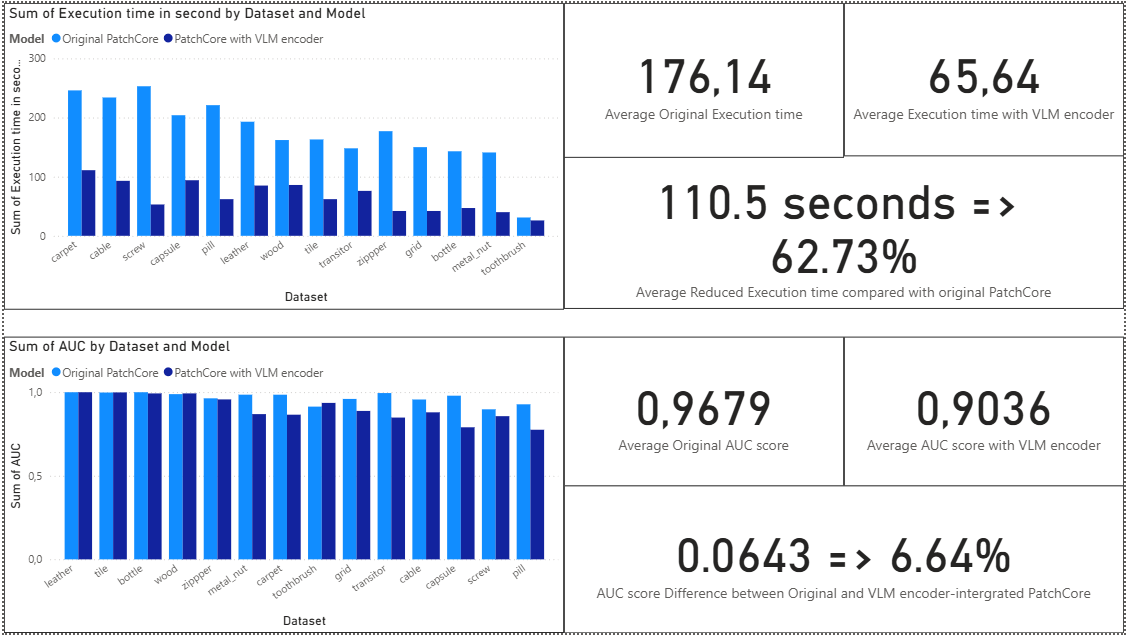
\includegraphics[width=0.7\linewidth]{images/analysis.png}
    \caption{Comparison between PatchCore with CNN and VLM backbone}
\end{figure}
    
\end{frame}
\begin{frame}{Next Steps to Add Text and Local Features Extraction into Training Phase}
\begin{block}{Idea}
    \begin{itemize}
        \item Currently only extracting the global image embeddings from CLIP, not the patch-level local ones in new pipeline.
        \item Already using CLIP encoder in training phase => able to encode natural language prompts like: "a normal bottle", "a defect-free metal surface", "a normal cable without damage",...
        \item These text embeddings live in the same space as the image embeddings because CLIP was trained to align them.
    \end{itemize}
\end{block}    
\end{frame}
\begin{frame}{Next Steps to Add Text into Training Phase}
\begin{block}{Potential Procedure}
    \begin{itemize}
        \item Add these text embeddings into the memory bank after being extracted and normalized using CLIP encoder.
        \item Text and image go through the different encoder:
        \begin{itemize}
            \item Images → image encoder
            \item Text → text encoder
        \end{itemize}
        \item Their outputs are aligned into the same vector space, so they can be stored in the same memory bank, as CLIP is trained so that image embeddings and text embeddings live in the same vector space.
        \item In testing phase, when we compare a test patch against the memory bank, it will be compared not only to other normal image patches, but also to semantic anchors from text.
    \end{itemize}
\end{block}    
\end{frame}